\section{Maquette de l'interface web}

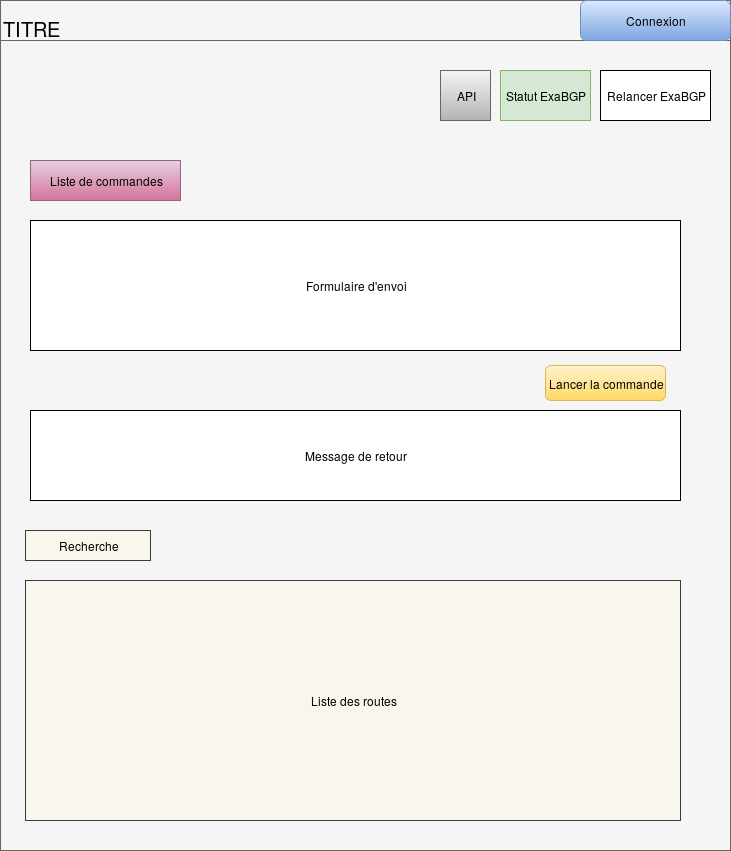
\includegraphics[scale=0.5]{img/maquette.png}
\\
Le bouton connexion permet à l'administrateur de se connecter en entrant son login/email et son mot de passe.\\
Le bouton "API" sert à rediriger vers l'API de ExaBGP à l'url suivant:
\\\url{https://github.com/Exa-Networks/exabgp/wiki/Controlling-ExaBGP-:-interacting-from-the-API}\\
La fonctionnalité "Statut ExaBGP" sert à afficher si ExaBGP fonctionne ou non.\\
Le bouton liste de commande permet de sélectionner la commande d'ExaBGP voulue.\\
En fonction de la commande sélectionnée un formulaire spécifique est affiché. Cette partie sera affichée dans les cas où la commande a besoin de paramètre.\\
Le bouton "lancer commande" permet d’exécuter la commande sur ExaBGP ou sur la base de donnée.\\
Une zone dédiée au retour de message de la commande lancé. Le message devra être le plus détaillé possible surtout pour les messages d'erreur d'une fonction qui s'est mal exécutée.\\
Une barre de recherche qui permettra à l'utilisateur ou à l'administrateur d'effectuer une recherche par préfixe d'adresse ip.\\
Une zone d'affichage qui listera la liste des routes. Initialement cette liste affichera les plus récentes routes stocké dans la base de donnée, mais si l'utilisateur effectue une recherche, c'est cette recherche qui sera affichée dans cette zone.